\documentclass{standalone}
\usepackage{tikz}
\usetikzlibrary{patterns, positioning}

\begin{document}
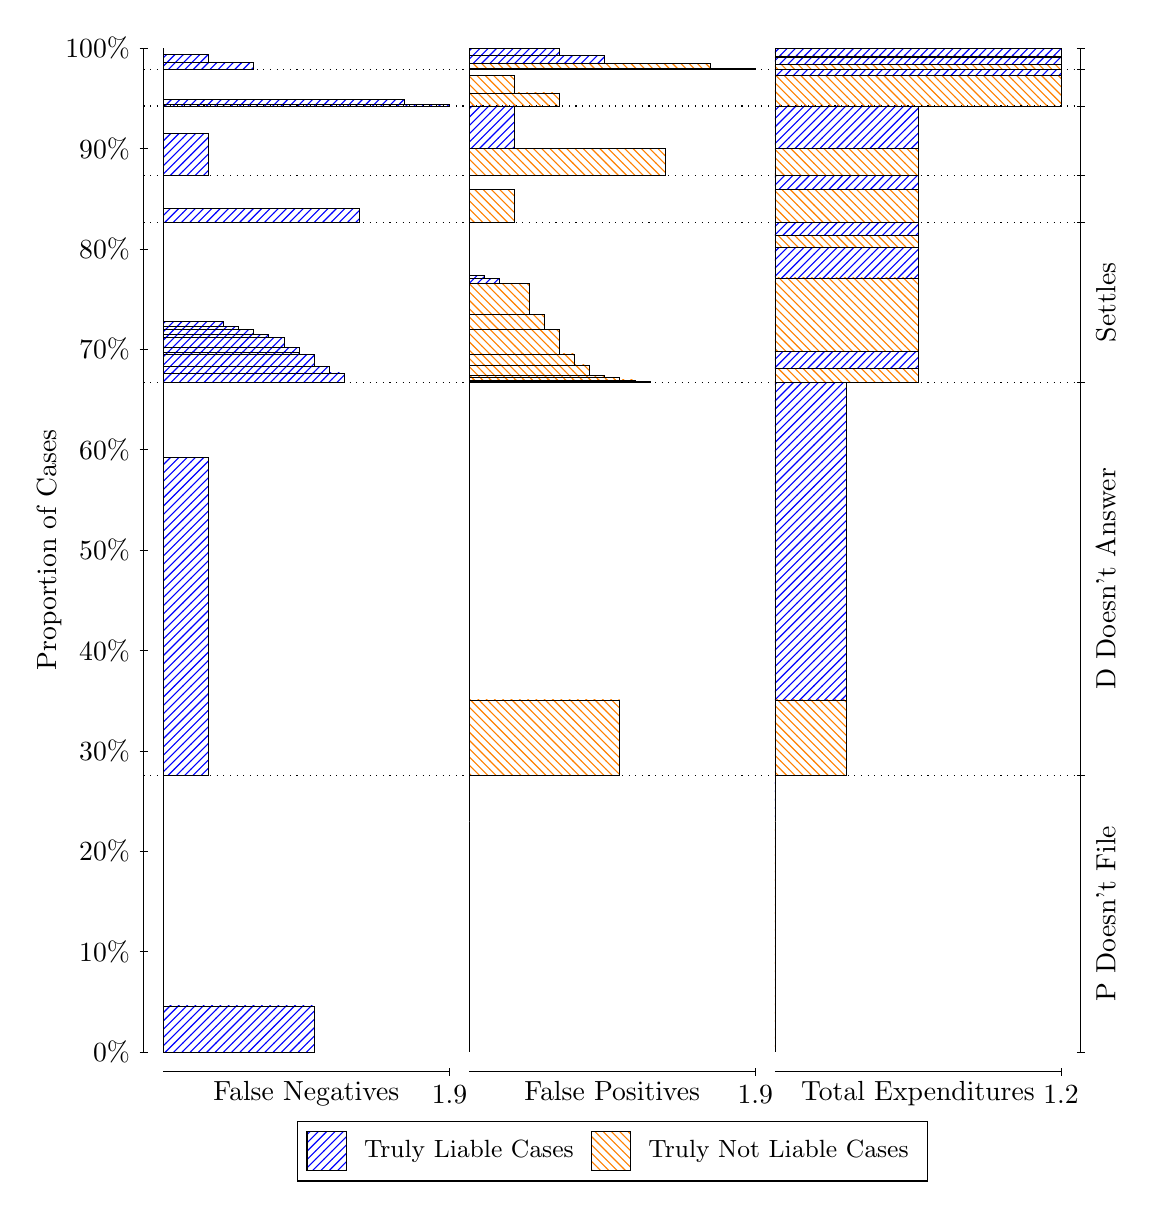
\begin{tikzpicture}
\draw[black, very thin] (1.5,1.75) -- (1.5,14.5);
\node[rotate=90, anchor=center] at (0.3, 8.125) {Proportion of Cases};
\draw[black, very thin] (1.45,1.75) -- (1.55,1.75);
\node[anchor=east] at (1.45, 1.75) {0\%};
\draw[black, very thin] (1.45,3.025) -- (1.55,3.025);
\node[anchor=east] at (1.45, 3.025) {10\%};
\draw[black, very thin] (1.45,4.3) -- (1.55,4.3);
\node[anchor=east] at (1.45, 4.3) {20\%};
\draw[black, very thin] (1.45,5.575) -- (1.55,5.575);
\node[anchor=east] at (1.45, 5.575) {30\%};
\draw[black, very thin] (1.45,6.85) -- (1.55,6.85);
\node[anchor=east] at (1.45, 6.85) {40\%};
\draw[black, very thin] (1.45,8.125) -- (1.55,8.125);
\node[anchor=east] at (1.45, 8.125) {50\%};
\draw[black, very thin] (1.45,9.4) -- (1.55,9.4);
\node[anchor=east] at (1.45, 9.4) {60\%};
\draw[black, very thin] (1.45,10.675) -- (1.55,10.675);
\node[anchor=east] at (1.45, 10.675) {70\%};
\draw[black, very thin] (1.45,11.95) -- (1.55,11.95);
\node[anchor=east] at (1.45, 11.95) {80\%};
\draw[black, very thin] (1.45,13.225) -- (1.55,13.225);
\node[anchor=east] at (1.45, 13.225) {90\%};
\draw[black, very thin] (1.45,14.5) -- (1.55,14.5);
\node[anchor=east] at (1.45, 14.5) {100\%};

\draw[black, very thin] (13.4,1.75) -- (13.4,14.5);
\draw[black, very thin] (13.35,1.75) -- (13.45,1.75);
\node[anchor=west] at (13.35, 1.75) {};
\draw[black, very thin] (13.35,5.2631) -- (13.45,5.2631);
\node[anchor=west] at (13.35, 5.2631) {};
\draw[black, very thin] (13.35,10.255) -- (13.45,10.255);
\node[anchor=west] at (13.35, 10.255) {};
\draw[black, very thin] (13.35,12.287) -- (13.45,12.287);
\node[anchor=west] at (13.35, 12.287) {};
\draw[black, very thin] (13.35,12.883) -- (13.45,12.883);
\node[anchor=west] at (13.35, 12.883) {};
\draw[black, very thin] (13.35,13.764) -- (13.45,13.764);
\node[anchor=west] at (13.35, 13.764) {};
\draw[black, very thin] (13.35,14.229) -- (13.45,14.229);
\node[anchor=west] at (13.35, 14.229) {};
\draw[black, very thin] (13.35,14.5) -- (13.45,14.5);
\node[anchor=west] at (13.35, 14.5) {};

\draw[black, very thin, pattern color=blue, pattern=north east lines] (1.75,1.75) rectangle (3.6623,2.3357);
\draw[black, very thin, pattern color=orange, pattern=north west lines] (1.75,2.3357) rectangle (1.75,5.2631);
\draw[black, very thin, pattern color=blue, pattern=north east lines] (1.75,5.2631) rectangle (2.3237,9.2969);
\draw[black, very thin, pattern color=orange, pattern=north west lines] (1.75,9.2969) rectangle (1.75,10.255);
\draw[black, very thin, pattern color=blue, pattern=north east lines] (1.75,10.255) rectangle (4.0447,10.373);
\draw[black, very thin, pattern color=blue, pattern=north east lines] (1.75,10.373) rectangle (3.8535,10.453);
\draw[black, very thin, pattern color=blue, pattern=north east lines] (1.75,10.453) rectangle (3.6623,10.612);
\draw[black, very thin, pattern color=blue, pattern=north east lines] (1.75,10.612) rectangle (3.4711,10.64);
\draw[black, very thin, pattern color=blue, pattern=north east lines] (1.75,10.64) rectangle (3.4711,10.702);
\draw[black, very thin, pattern color=blue, pattern=north east lines] (1.75,10.702) rectangle (3.2798,10.827);
\draw[black, very thin, pattern color=blue, pattern=north east lines] (1.75,10.827) rectangle (3.0886,10.867);
\draw[black, very thin, pattern color=blue, pattern=north east lines] (1.75,10.867) rectangle (2.8974,10.93);
\draw[black, very thin, pattern color=blue, pattern=north east lines] (1.75,10.93) rectangle (2.7061,10.965);
\draw[black, very thin, pattern color=blue, pattern=north east lines] (1.75,10.965) rectangle (2.5149,11.027);
\draw[black, very thin, pattern color=orange, pattern=north west lines] (1.75,11.027) rectangle (1.75,12.287);
\draw[black, very thin, pattern color=blue, pattern=north east lines] (1.75,12.287) rectangle (4.236,12.462);
\draw[black, very thin, pattern color=orange, pattern=north west lines] (1.75,12.462) rectangle (1.75,12.883);
\draw[black, very thin, pattern color=blue, pattern=north east lines] (1.75,12.883) rectangle (2.3237,13.419);
\draw[black, very thin, pattern color=orange, pattern=north west lines] (1.75,13.419) rectangle (1.75,13.764);
\draw[black, very thin, pattern color=blue, pattern=north east lines] (1.75,13.764) rectangle (5.3833,13.789);
\draw[black, very thin, pattern color=blue, pattern=north east lines] (1.75,13.789) rectangle (4.8096,13.844);
\draw[black, very thin, pattern color=orange, pattern=north west lines] (1.75,13.844) rectangle (1.75,14.229);
\draw[black, very thin, pattern color=blue, pattern=north east lines] (1.75,14.229) rectangle (2.8974,14.322);
\draw[black, very thin, pattern color=blue, pattern=north east lines] (1.75,14.322) rectangle (2.3237,14.421);
\draw[black, very thin, pattern color=orange, pattern=north west lines] (1.75,14.421) rectangle (1.75,14.5);
\draw[black, very thin, pattern color=orange, pattern=north west lines] (5.6333,1.75) rectangle (5.6333,4.6773);
\draw[black, very thin, pattern color=blue, pattern=north east lines] (5.6333,4.6773) rectangle (5.6333,5.2631);
\draw[black, very thin, pattern color=orange, pattern=north west lines] (5.6333,5.2631) rectangle (7.5456,6.221);
\draw[black, very thin, pattern color=blue, pattern=north east lines] (5.6333,6.221) rectangle (5.6333,10.255);
\draw[black, very thin, pattern color=orange, pattern=north west lines] (5.6333,10.255) rectangle (7.9281,10.27);
\draw[black, very thin, pattern color=orange, pattern=north west lines] (5.6333,10.27) rectangle (7.7368,10.285);
\draw[black, very thin, pattern color=orange, pattern=north west lines] (5.6333,10.285) rectangle (7.5456,10.314);
\draw[black, very thin, pattern color=orange, pattern=north west lines] (5.6333,10.314) rectangle (7.3544,10.345);
\draw[black, very thin, pattern color=orange, pattern=north west lines] (5.6333,10.345) rectangle (7.1632,10.475);
\draw[black, very thin, pattern color=orange, pattern=north west lines] (5.6333,10.475) rectangle (6.9719,10.615);
\draw[black, very thin, pattern color=orange, pattern=north west lines] (5.6333,10.615) rectangle (6.7807,10.925);
\draw[black, very thin, pattern color=orange, pattern=north west lines] (5.6333,10.925) rectangle (6.5895,11.12);
\draw[black, very thin, pattern color=orange, pattern=north west lines] (5.6333,11.12) rectangle (6.3982,11.515);
\draw[black, very thin, pattern color=blue, pattern=north east lines] (5.6333,11.515) rectangle (6.0158,11.577);
\draw[black, very thin, pattern color=blue, pattern=north east lines] (5.6333,11.577) rectangle (5.8246,11.612);
\draw[black, very thin, pattern color=blue, pattern=north east lines] (5.6333,11.612) rectangle (5.6333,12.287);
\draw[black, very thin, pattern color=orange, pattern=north west lines] (5.6333,12.287) rectangle (6.207,12.708);
\draw[black, very thin, pattern color=blue, pattern=north east lines] (5.6333,12.708) rectangle (5.6333,12.883);
\draw[black, very thin, pattern color=orange, pattern=north west lines] (5.6333,12.883) rectangle (8.1193,13.228);
\draw[black, very thin, pattern color=blue, pattern=north east lines] (5.6333,13.228) rectangle (6.207,13.764);
\draw[black, very thin, pattern color=orange, pattern=north west lines] (5.6333,13.764) rectangle (6.7807,13.93);
\draw[black, very thin, pattern color=orange, pattern=north west lines] (5.6333,13.93) rectangle (6.207,14.15);
\draw[black, very thin, pattern color=blue, pattern=north east lines] (5.6333,14.15) rectangle (5.6333,14.229);
\draw[black, very thin, pattern color=orange, pattern=north west lines] (5.6333,14.229) rectangle (9.2667,14.245);
\draw[black, very thin, pattern color=orange, pattern=north west lines] (5.6333,14.245) rectangle (8.693,14.308);
\draw[black, very thin, pattern color=blue, pattern=north east lines] (5.6333,14.308) rectangle (7.3544,14.408);
\draw[black, very thin, pattern color=blue, pattern=north east lines] (5.6333,14.408) rectangle (6.7807,14.5);
\draw[black, very thin, pattern color=orange, pattern=north west lines] (9.5167,1.75) rectangle (9.5167,4.6773);
\draw[black, very thin, pattern color=blue, pattern=north east lines] (9.5167,4.6773) rectangle (9.5167,5.2631);
\draw[black, very thin, pattern color=orange, pattern=north west lines] (9.5167,5.2631) rectangle (10.425,6.221);
\draw[black, very thin, pattern color=blue, pattern=north east lines] (9.5167,6.221) rectangle (10.425,10.255);
\draw[black, very thin, pattern color=orange, pattern=north west lines] (9.5167,10.255) rectangle (11.333,10.429);
\draw[black, very thin, pattern color=blue, pattern=north east lines] (9.5167,10.429) rectangle (11.333,10.652);
\draw[black, very thin, pattern color=orange, pattern=north west lines] (9.5167,10.652) rectangle (11.333,11.58);
\draw[black, very thin, pattern color=blue, pattern=north east lines] (9.5167,11.58) rectangle (11.333,11.966);
\draw[black, very thin, pattern color=orange, pattern=north west lines] (9.5167,11.966) rectangle (11.333,12.124);
\draw[black, very thin, pattern color=blue, pattern=north east lines] (9.5167,12.124) rectangle (11.333,12.287);
\draw[black, very thin, pattern color=orange, pattern=north west lines] (9.5167,12.287) rectangle (11.333,12.708);
\draw[black, very thin, pattern color=blue, pattern=north east lines] (9.5167,12.708) rectangle (11.333,12.883);
\draw[black, very thin, pattern color=orange, pattern=north west lines] (9.5167,12.883) rectangle (11.333,13.228);
\draw[black, very thin, pattern color=blue, pattern=north east lines] (9.5167,13.228) rectangle (11.333,13.764);
\draw[black, very thin, pattern color=orange, pattern=north west lines] (9.5167,13.764) rectangle (13.15,14.15);
\draw[black, very thin, pattern color=blue, pattern=north east lines] (9.5167,14.15) rectangle (13.15,14.229);
\draw[black, very thin, pattern color=orange, pattern=north west lines] (9.5167,14.229) rectangle (13.15,14.292);
\draw[black, very thin, pattern color=blue, pattern=north east lines] (9.5167,14.292) rectangle (13.15,14.384);
\draw[black, very thin, pattern color=orange, pattern=north west lines] (9.5167,14.384) rectangle (13.15,14.4);
\draw[black, very thin, pattern color=blue, pattern=north east lines] (9.5167,14.4) rectangle (13.15,14.5);
\draw[black, dotted] (1.5,5.2631) -- (13.4,5.2631);
\draw[black, dotted] (1.5,10.255) -- (13.4,10.255);
\draw[black, dotted] (1.5,12.287) -- (13.4,12.287);
\draw[black, dotted] (1.5,12.883) -- (13.4,12.883);
\draw[black, dotted] (1.5,13.764) -- (13.4,13.764);
\draw[black, dotted] (1.5,14.229) -- (13.4,14.229);
\draw[black, very thin] (1.75,1.5) -- (5.3833,1.5);
\node[anchor=north] at (3.5667, 1.5) {False Negatives};
\draw[black, very thin] (5.3833,1.45) -- (5.3833,1.55);
\node[anchor=north] at (5.3833, 1.45) {1.9};

\draw[black, very thin] (5.6333,1.5) -- (9.2667,1.5);
\node[anchor=north] at (7.45, 1.5) {False Positives};
\draw[black, very thin] (9.2667,1.45) -- (9.2667,1.55);
\node[anchor=north] at (9.2667, 1.45) {1.9};

\draw[black, very thin] (9.5167,1.5) -- (13.15,1.5);
\node[anchor=north] at (11.333, 1.5) {Total Expenditures};
\draw[black, very thin] (13.15,1.45) -- (13.15,1.55);
\node[anchor=north] at (13.15, 1.45) {1.2};

\node[black, centered, rotate=90] at (13.72, 3.5065) {P Doesn't File};
\node[black, centered, rotate=90] at (13.72, 7.7589) {D Doesn't Answer};
\node[black, centered, rotate=90] at (13.72, 11.271) {Settles};





\draw (7.449999999999999,1.5) node[draw=none] (baseCoordinate) {};
\begin{scope}[align=center]
        \matrix[scale=0.5, draw=black, below=0.5cm of baseCoordinate, nodes={draw}, column sep=0.1cm]{
            \node[rectangle, draw, minimum width=0.5cm, minimum height=0.5cm, pattern=north east lines, pattern color=blue] {}; &
            \node[draw=none, font=\small] (B) {Truly Liable Cases}; &
            \node[rectangle, draw, minimum width=0.5cm, minimum height=0.5cm, pattern=north west lines, pattern color=orange] {}; &
            \node[draw=none, font=\small] (B) {Truly Not Liable Cases}; \\
            };
\end{scope}

\end{tikzpicture}
\end{document}